\section{Data, Queries and Damage}
\label{sec:data}

\subsection{The graph}
\label{sec:data-graphs}

We use a fixed release of PrimeKG \cite{chandak2023primekg}
(file \texttt{kg.csv}, Harvard Dataverse file 6180620; checksums in
Appendix~\ref{app:repro}). We keep three entity types (drug, disease,
gene/protein) and three relations (drug--protein, disease--protein,
protein--protein). Reverse and duplicate records are merged into one undirected
edge per entity pair, and self-loops are removed. This filtered graph, which we
call the full graph, has 30,968 nodes and 426,954 edges. No entity pair carries
more than one relation, so the routes between a drug and a disease through
different proteins share no edge, which Section~\ref{sec:theory-r2} uses.

\subsection{Queries: approved indications and decoys}
\label{sec:data-indications}

A query $(d,y)$ asks whether drug $d$ and disease $y$ are linked through
proteins. It succeeds at hop limit $L$ if there is a typed path
\begin{equation*}
d \xrightarrow{\text{drug--protein}} x_1 \xrightarrow{\text{PPI}} \cdots
\xrightarrow{\text{PPI}} x_j \xrightarrow{\text{disease--protein}} y,
\qquad j-1\le L-2,
\end{equation*}
with $j-1$ protein--protein (PPI) steps. For $L=2$ the drug and disease must share
a protein, and the number $m$ of shared proteins is the query's redundancy
(Figure~\ref{fig:schematic}).

\begin{figure}[!htbp]
  \centering
  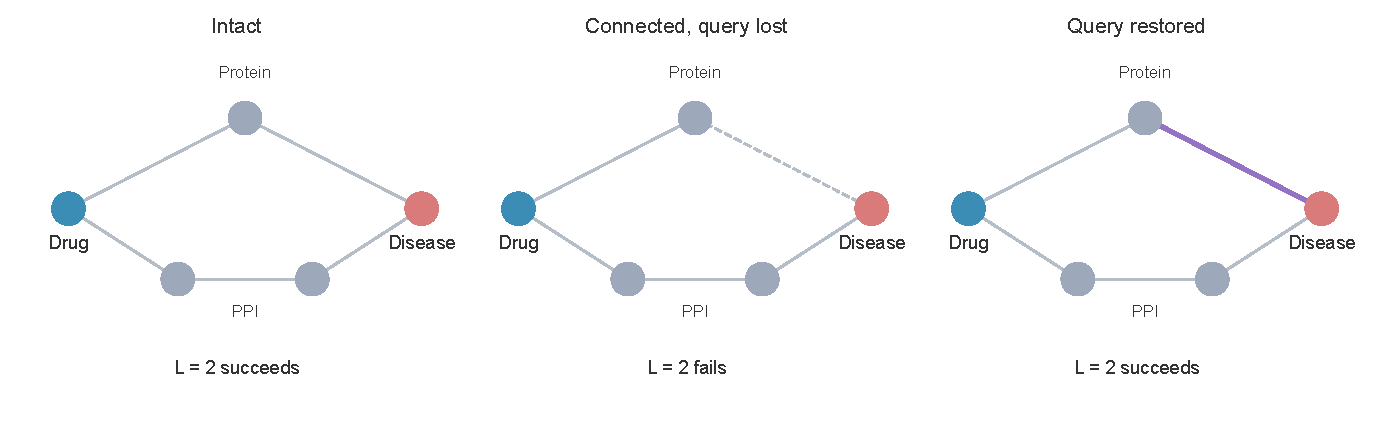
\includegraphics[width=0.86\linewidth]{act0/fig_query_schematic.pdf}
  \caption{A typed query. Left: the drug and the disease share a protein, so the
  query succeeds at $L=2$; a longer route through two interacting proteins also
  exists. Middle: losing one disease--protein link leaves the pair connected, but
  the two-hop answer is gone, which is the situation of this report's title.
  Right: restoring that link recovers it (Appendix~\ref{sec:repair}).}
  \label{fig:schematic}
\end{figure}

The main queries are PrimeKG's approved drug indications. PrimeKG lists 9,388
drug--disease indication pairs, and for 6,233 of them both endpoints are in the
full graph. These pairs are not part of the graph we damage, because only
drug--protein, disease--protein and protein--protein edges were kept, so they
are evidence that the retrieval rule has not seen. For each indication we form a
decoy by permuting the diseases among the indicated drugs and rejecting any pair
that PrimeKG lists as an indication, a contraindication or an off-label use.
Every decoy keeps the drug of one indication and the decoy diseases are the
indicated diseases in a new order, so the two sets have almost identical
distributions of drug and disease degree. We report the recall (the share of
indications with a typed path within $L$ hops), the decoy rate (the same share
for decoys), their ratio, and the mutual information in bits between the label
and the retrieval outcome for a balanced mixture of the two sets. Of the
indications, 1,931 have at least one shared protein; we call them two-hop
indications. Our first benchmark drew its queries from the graph we were
damaging, so it could tell us whether paths survive but not whether they mean
anything. Indications that the damaged graph does not contain turned a
robustness exercise into the question of this report.

\subsection{A controlled testbed}
\label{sec:data-sample}

To test the theory under full control, we also use the induced subgraph on the
first 5,000 nodes reached by breadth-first search (BFS) from the disease of
highest degree, with ties broken by index, which we call the sample. Its
benchmark has 200 drug--disease queries that succeed at $L=2$: 100 with $m=1$
and 100 with $m\ge2$, drawn with a fixed seed from the 3,175 and 1,264 such
pairs. They involve 39 drugs and 127 diseases. The 50/50 mix sets the level of
$R_2$, so the benchmark's success rates describe this controlled task, not
PrimeKG. Table~\ref{tab:graphs} compares the two graphs.

\begin{table}[!htbp]
\centering
\small
\caption{Graphs used in this report. Assortativity $r$ is the degree
correlation across edges \cite{newman2002assortative}. The last column is the mean degree of the neighbors of nodes with degree at most 3, averaged over
their edges. For an uncorrelated graph with the same degrees it would be
$\langle k^2\rangle/\langle k\rangle$, which is 189 for the sample and 190 for the full graph.}
\label{tab:graphs}
\begin{tabular}{@{}lrrrrrrrr@{}}
\toprule
Graph & Nodes & Edges & Drugs & Diseases & Proteins & $\langle k\rangle$ & $r$ & Neighbor degree \\
\midrule
BFS sample & 5,000 & 117,891 & 74 & 283 & 4,643 & 47.2 & $-0.153$ & 486 \\
Full graph & 30,968 & 426,954 & 6,282 & 5,593 & 19,093 & 27.6 & $-0.053$ & 209 \\
\bottomrule
\end{tabular}
\end{table}

The sample has 90,187 protein--protein, 27,228 disease--protein and
only 476 drug--protein edges. Proteins make up 93\% of its nodes. Of its 74
drugs, 51 have a single target.

\paragraph{The sample is not PrimeKG.} BFS reaches peripheral nodes through
hubs, and a node at the frontier keeps only its edges into nodes already
visited. The sample therefore has a denser core than the full graph, and its
low-degree nodes hang from hubs. Table~\ref{tab:graphs} shows this directly. In
the full graph, low-degree nodes have neighbors only slightly more connected
than in an uncorrelated graph (209 against 190), and the assortativity is
$-0.053$. In the sample these values are 486 and $-0.153$. The sample's median
degree is 25 and only 2\% of its nodes have a single edge; in the full graph
these are 9 and 22\%. The sample is therefore a testbed for the theory, not a
model of PrimeKG, and we state which conclusions concern it only.

\subsection{Damage and observables}
\label{sec:data-damage}

Under blind damage, a fraction $f$ of edges or nodes is removed in a random
order; removing a node also removes its edges. We write $p=1-f$ for edge
retention and $\phi=1-f$ for node retention. For targeted damage, nodes are
removed in decreasing order of degree, or of betweenness centrality estimated
from 100 sampled sources (seed 42); both rankings are computed once on the
intact graph. The giant component $S(f)$ is the share of the original nodes in
the largest connected component. Retrieval success $R_L(f)$ is the share of
queries that still have a typed path of at most $L$ hops; a query whose drug or
disease has been removed fails.

Expected values under blind damage are Monte Carlo means over independent damage
orders: on the sample, 5,000 orders when two-hop retrieval is compared with
Eq.~\eqref{eq:r2} and 600 for scans over the hop limit; on the full graph, 500
orders for the two-hop indications of Figure~\ref{fig:summary}a and five orders
for all other scans, including the comparisons of all indications with decoys. Ten fixed orders (seeds 0--9) are used
where a stored damage state is needed and to show the spread of a single damage
state. Each order is a random permutation, and the damage state at fraction $f$
is its first $\mathrm{round}(fE)$ entries. Targeted removal is deterministic.
